\documentclass[conf]{new-aiaa}

\usepackage[utf8]{inputenc}
\usepackage{amsmath}
\usepackage{graphicx}
\usepackage{array}
\usepackage{longtable,tabularx}
\usepackage{booktabs}
\usepackage{multirow}
\usepackage{float}
\usepackage{hyperref}
\usepackage{caption}
\usepackage{enumitem}

\setlength\LTleft{0pt}
\captionsetup[table]{position=bottom,skip=6pt}
\captionsetup[figure]{position=bottom,skip=6pt}
\newcolumntype{Y}{>{\raggedright\arraybackslash}X}

\begin{document}
\begin{titlepage}
    \centering
    \vspace*{1.5cm}

    {\LARGE \textbf{TAMU-SPIRIT System Requirements Review Report}\par}
    \vspace{0.2cm}
    {\large \textbf{System Requirements Review (SRR)}\par}

    \vspace{0.6cm}
    \rule{0.8\textwidth}{0.4pt}\par
    \vspace{0.6cm}

    {\large AERO 401 Capstone \textbar\ Section 930\par}
    {\large Department of Aerospace Engineering\par}
    {\large Texas A\&M University\par}
    {\large Spring 2026\par}

    \vspace{0.8cm}
    {\large \textbf{Team Members}\par}
    \vspace{0.3cm}
    \begin{tabular}{@{}p{0.48\textwidth}p{0.48\textwidth}@{}}
    Sophia Cuellar \hfill 832006961 & Noah Matus \hfill 732007548 \\
    Aiden Kampwerth \hfill 632003715 & Riley McNew \hfill 234001693 \\
    Steven Minniear \hfill 233009885 & Vin Manoj Nair \hfill 833006608 \\
    Param Patel \hfill 332002218 & Matthew Thanjan \hfill 732004647 \\
    \end{tabular}

    \vspace{0.8cm}
    {\large \textbf{Faculty Advisor:} John Connolly\par}
    {\large \textbf{Revision:} Final v1.0\par}
    {\large \textbf{Prepared on:} \today\par}

    \vspace*{\fill}
\end{titlepage}

\tableofcontents
\clearpage
\listoftables
\clearpage


\section*{Team Contributions}
\addcontentsline{toc}{section}{Team Contributions}
\begin{table}[!htbp]
    \centering
    \footnotesize
    \setlength{\tabcolsep}{4pt}
    \renewcommand{\arraystretch}{1.15}
    \begin{tabularx}{\textwidth}{@{}>{\raggedright\arraybackslash}p{3.2cm}
                                    >{\raggedright\arraybackslash}X
                                    >{\raggedright\arraybackslash}X
                                    >{\centering\arraybackslash}p{2.0cm}
                                    >{\centering\arraybackslash}p{2.0cm}@{}}
    \toprule
    \textbf{Team Member} & \textbf{Sections Contributed} & \textbf{Sections Reviewed} & \textbf{Total Words} & \textbf{Total Graphics} \\
    \midrule
    Sophia Cuellar & \S4 & \S2, \S4 & 964 & 0 \\
    Aiden Kampwerth & \S5, \S4 & \S4 & 1051 & 0 \\
    Noah Matus & \S1, \S4 & \S3, \S4 & 1316 & 0 \\
    Riley McNew & \S4 & \S4 & 564 & 0 \\
    Steven Minniear & \S2, \S4 & \S4-5 & 1340 & 2 \\
    Vin Manoj Nair & \S2, \S4 & \S4, \S6 & 899 & 1 \\
    Param Patel & \S1, \S4 & \S4, \S6 & 893 & 0 \\
    Matthew Thanjan & \S4 & \S1, \S5 & 361 & 0 \\
    \bottomrule
    \end{tabularx}
\end{table}
\clearpage
\section{System Goals \& Success Criteria}


The TAMU SPIRIT system goals and success criteria present in Table~\ref{tab:system_goals} define the high-level conditions under which the TAMU-SPIRIT program will be considered successful at the platform level, independent of any individual flight experiment. These goals were derived from stakeholder needs and the TAMU-SPIRIT program and shall serve as a foundation against which all experiment design decisions are evaluated.

\begin{table}[!htbp]
    \centering
    \footnotesize
    \setlength{\tabcolsep}{4pt}
    \renewcommand{\arraystretch}{1.15}
    \begin{tabularx}{\textwidth}{@{}>{\centering\arraybackslash}m{1.9cm}
                                    >{\raggedright\arraybackslash}p{6.1cm}
                                    >{\raggedright\arraybackslash}p{3.3cm}
                                    >{\raggedright\arraybackslash}p{3.3cm}@{}}
    \toprule
    \textbf{Goal ID and Priority} & \textbf{Goal} & \textbf{Metric} & \textbf{Target Value} \\
    \midrule
    \shortstack[c]{\textbf{SG-1}\\Critical} &
    The TAMU-SPIRIT system shall provide dedicated priority access to the ISS exterior environment for Texas A\&M University System researchers, faculty, and students, enabling experiments that cannot be conducted in ground-based facilities. &
    The number of flight experiments sent aboard the TAMU-SPIRIT facility. &
    $\geq$1 flight experiment is sent aboard the TAMU-SPIRIT facility. \\

    \shortstack[c]{\textbf{SG-2}\\Critical} &
    The TAMU-SPIRIT system shall support high-quality scientific and technical research that addresses meaningful challenges. &
    Number of PI-defined research objectives supported by collecting data. &
    $\geq$ 1 primary research objective successfully achieved. \\

    \shortstack[c]{\textbf{SG-3}\\Critical} &
    The TAMU-SPIRIT system shall successfully operate externally mounted Science Carriers and Pallet Carriers to enable multi-user research. &
    The number of Science and Pallet Carrier that successfully provides the required power and data throughout the mission. &
    All experiments receive the required power and data throughout the mission. \\

    \shortstack[c]{\textbf{SG-4}\\Critical} &
    The TAMU-SPIRIT system shall provide end-to-end mission services, including launch to the ISS, on-orbit operations, and return of experiment hardware to Earth. &
    The number of Flight experiments operated for the full mission duration with no anomalies, and all samples were returned to Earth. &
    All flight experiments operate for the full mission duration with no anomalies, and all samples are returned to Earth. \\

    \shortstack[c]{\textbf{SG-5}\\Critical} &
    The TAMU-SPIRIT system shall serve as a platform to build a strategic research partnership between Texas A\&M University and an external academic institution. &
    The number of research partnerships established with multiple external institutions &
    $\geq$ 1 partnership established. \\
    \bottomrule
    \end{tabularx}
    \caption{System Goals and Success Criteria}
    \label{tab:system_goals}
\end{table}

\clearpage
\section{System Concepts and Architecture}

The Texas A\&M Space Platform Integrating Research and Innovative Technology (TAMU-SPIRIT) is an externally mounted multi-payload flight facility deployed on the International Space Station (ISS), developed in partnership with Aegis Aerospace. The facility is designed around a modular carrier-based system, which is capable of hosting up to twelve Science Carriers or Pallet Carriers simultaneously. Each will provide standardized mechanical, electrical, and data interfaces to hosted flight experiments. TAMU-SPIRIT operates in a Low Earth Orbit environment at the ISS orbital altitude of approximately 400 km, subjecting externally mounted payloads to atomic oxygen flux, radiation, hard vacuum, and thermal cycling between approximately $-120\,^{\circ}$C and $+120\,^{\circ}$C across each 90 minute orbital period. The facility supports multi-experiment operations for deployment cycles of six to twelve months, after which all carriers and experiment hardware are returned to Earth via SpaceX Dragon for post-flight analysis.

TAMU-SPIRIT allows a maximum of twelve payload carriers at a time, with each carrier assigned a designated position on the facility's external mounting structure to which mechanical, electrical, and data connections are made. Science Carriers (SC) are restricted to a single dimension of 298.45 mm $\times$ 168.91 mm $\times$ 79.375 mm with a weight limit of 10 kg, whereas Pallet Carriers (PC) have a larger dimension limit of 421.64 mm $\times$ 218.44 mm $\times$ 250.69 mm with a weight limit of 20 kg. Each carrier slot receives up to 75 W of electrical power at 28V DC, and all data, with a maximum of 5 Mbps downlink and 2 Mbps uplink, is transferred daily at a downlink limit of 1 GB and an uplink limit of 100 MB during the work week. Depending on the scientific goals of the experiment, any of the Carriers may be positioned in the Ram, Wake, Nadir, or Zenith directions. Carriers facing RAM will undergo increased atomic oxygen flux due to direct exposure while traveling along the ISS velocity vector. Wake facing carriers will operate in a virtually ideal vacuum, Nadir carriers will have a constant line of sight to the Earth, and Zenith will look toward outer space. All interfaces of carriers shall be verified by Aegis Aerospace before the flight integration stage.

Currently, the team is collaborating with ten candidate flight experiments. Each is sponsored by one of the project's Principal Investigators (PI), whose research goals should define the scientific and technical specifications of the payload. Current experiments include Rat Kidney Cryopreservation, Phage Biofilm, Self-Healing Polymer Exposure, Additive Manufacturing Exposure, Heat Sensor Exposure, Fungal Spore Exposure, Freeze-Dried Food Analog, Plume Detection, and Star Tracker Gimbal. The TAMU-SPIRIT mission's primary objective is to provide an operational space to validate the research claims of each PI by conducting experiments that are not possible to execute on Earth. These studies span from the behavior of biological materials in microgravity, the degradation of materials during extended exposure to space, and the reliability of autonomous sensing systems.

\begin{figure}[H]
    \centering
    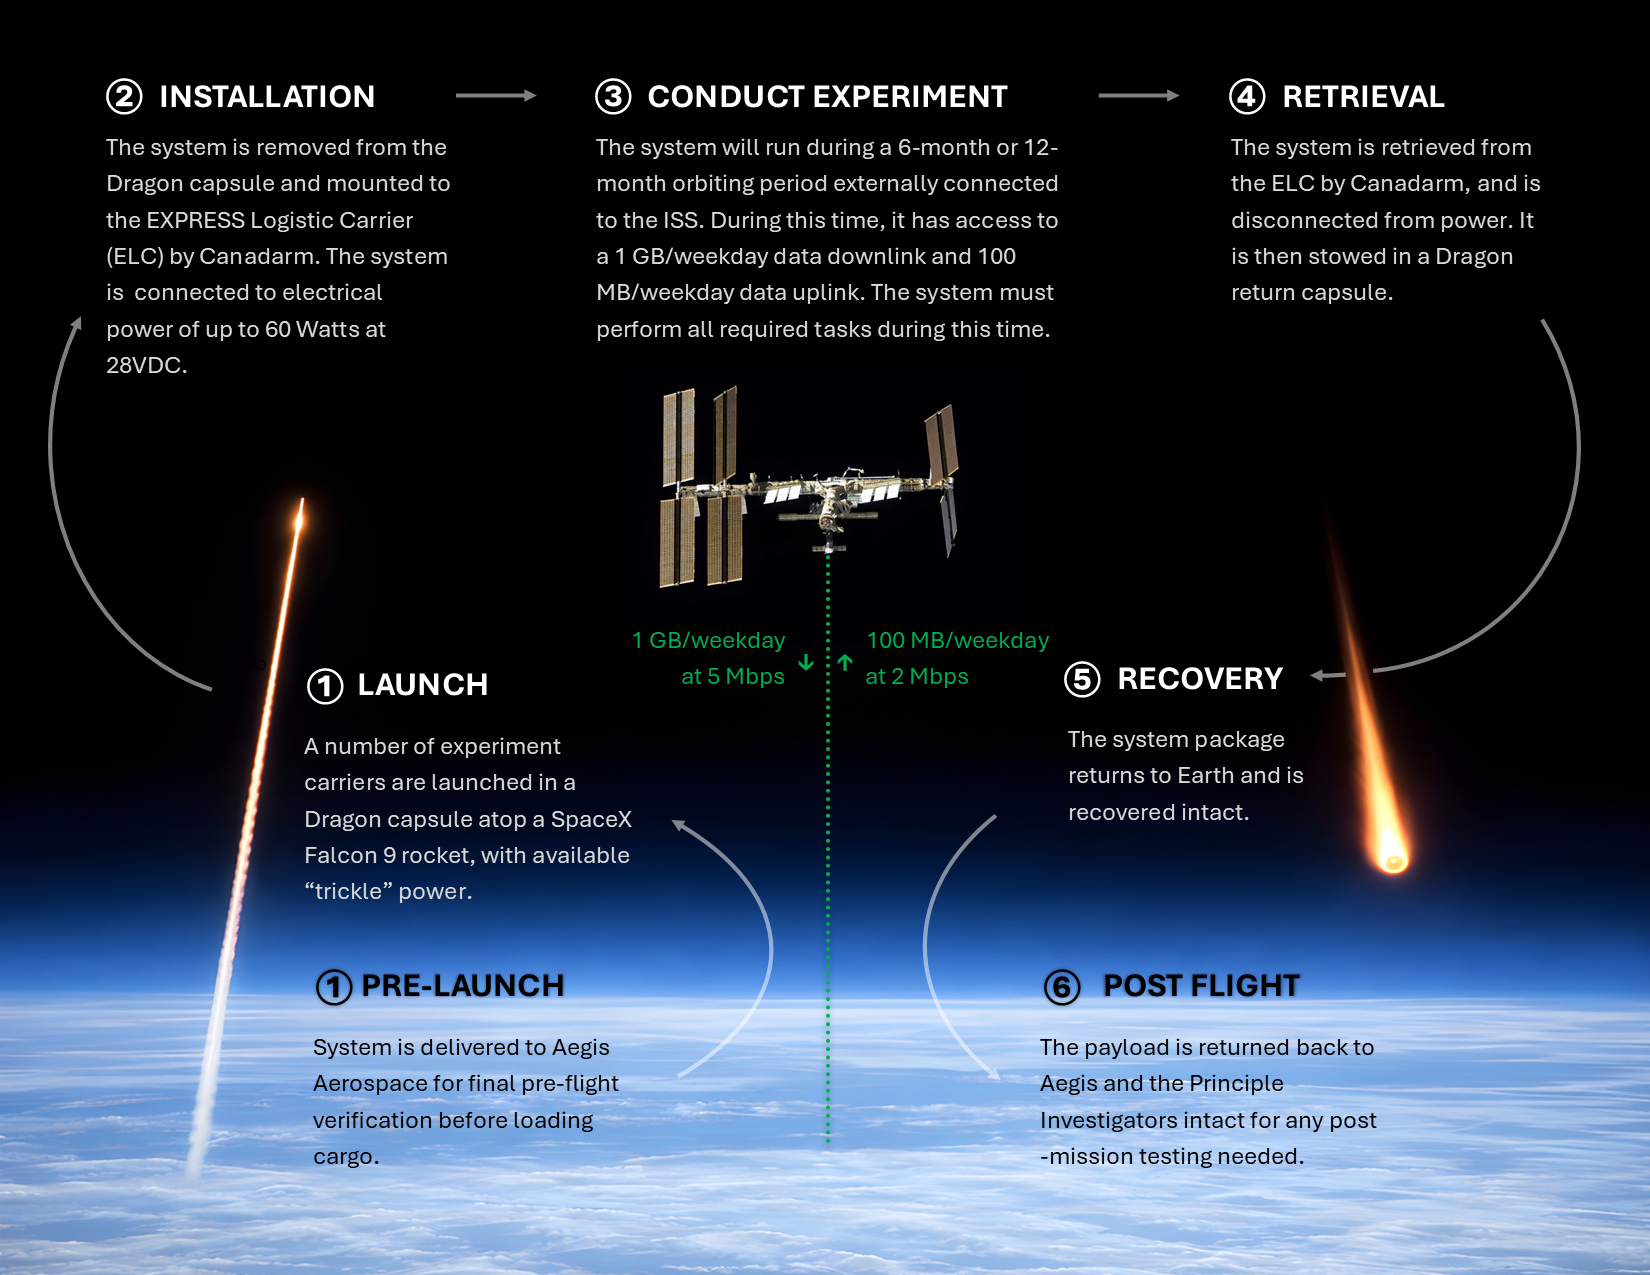
\includegraphics[width=\linewidth,height=0.78\textheight,keepaspectratio]{conops_new.png}
    \caption{TAMU-SPIRIT ConOps Overview}
    \label{fig:conops_new}
\end{figure}

Following the System Concept Review, the team focused on defining the requirements for the individual flight experiments and started formulating some preliminary solutions to the principal engineering problems common to the candidate portfolio. For example, in order to maintain a specified temperature, the team is considering the use of resistive heaters and cooling devices that will allow for active temperature control of the carriers. In terms of the design for the storage and protection of biological samples from the effects of radiation, the team is evaluating the use of radiation-tolerant materials as a form of passive shielding. To ensure there is no risk of biological contamination to the environment of the ISS, the team is considering the use of closed, tight vacuum-sealed containers for all experiments that will involve biological materials. These concepts will be expanded during the upcoming detailed design phase, which will go into more depth in the PDR.

\begin{figure}[H]
    \centering
    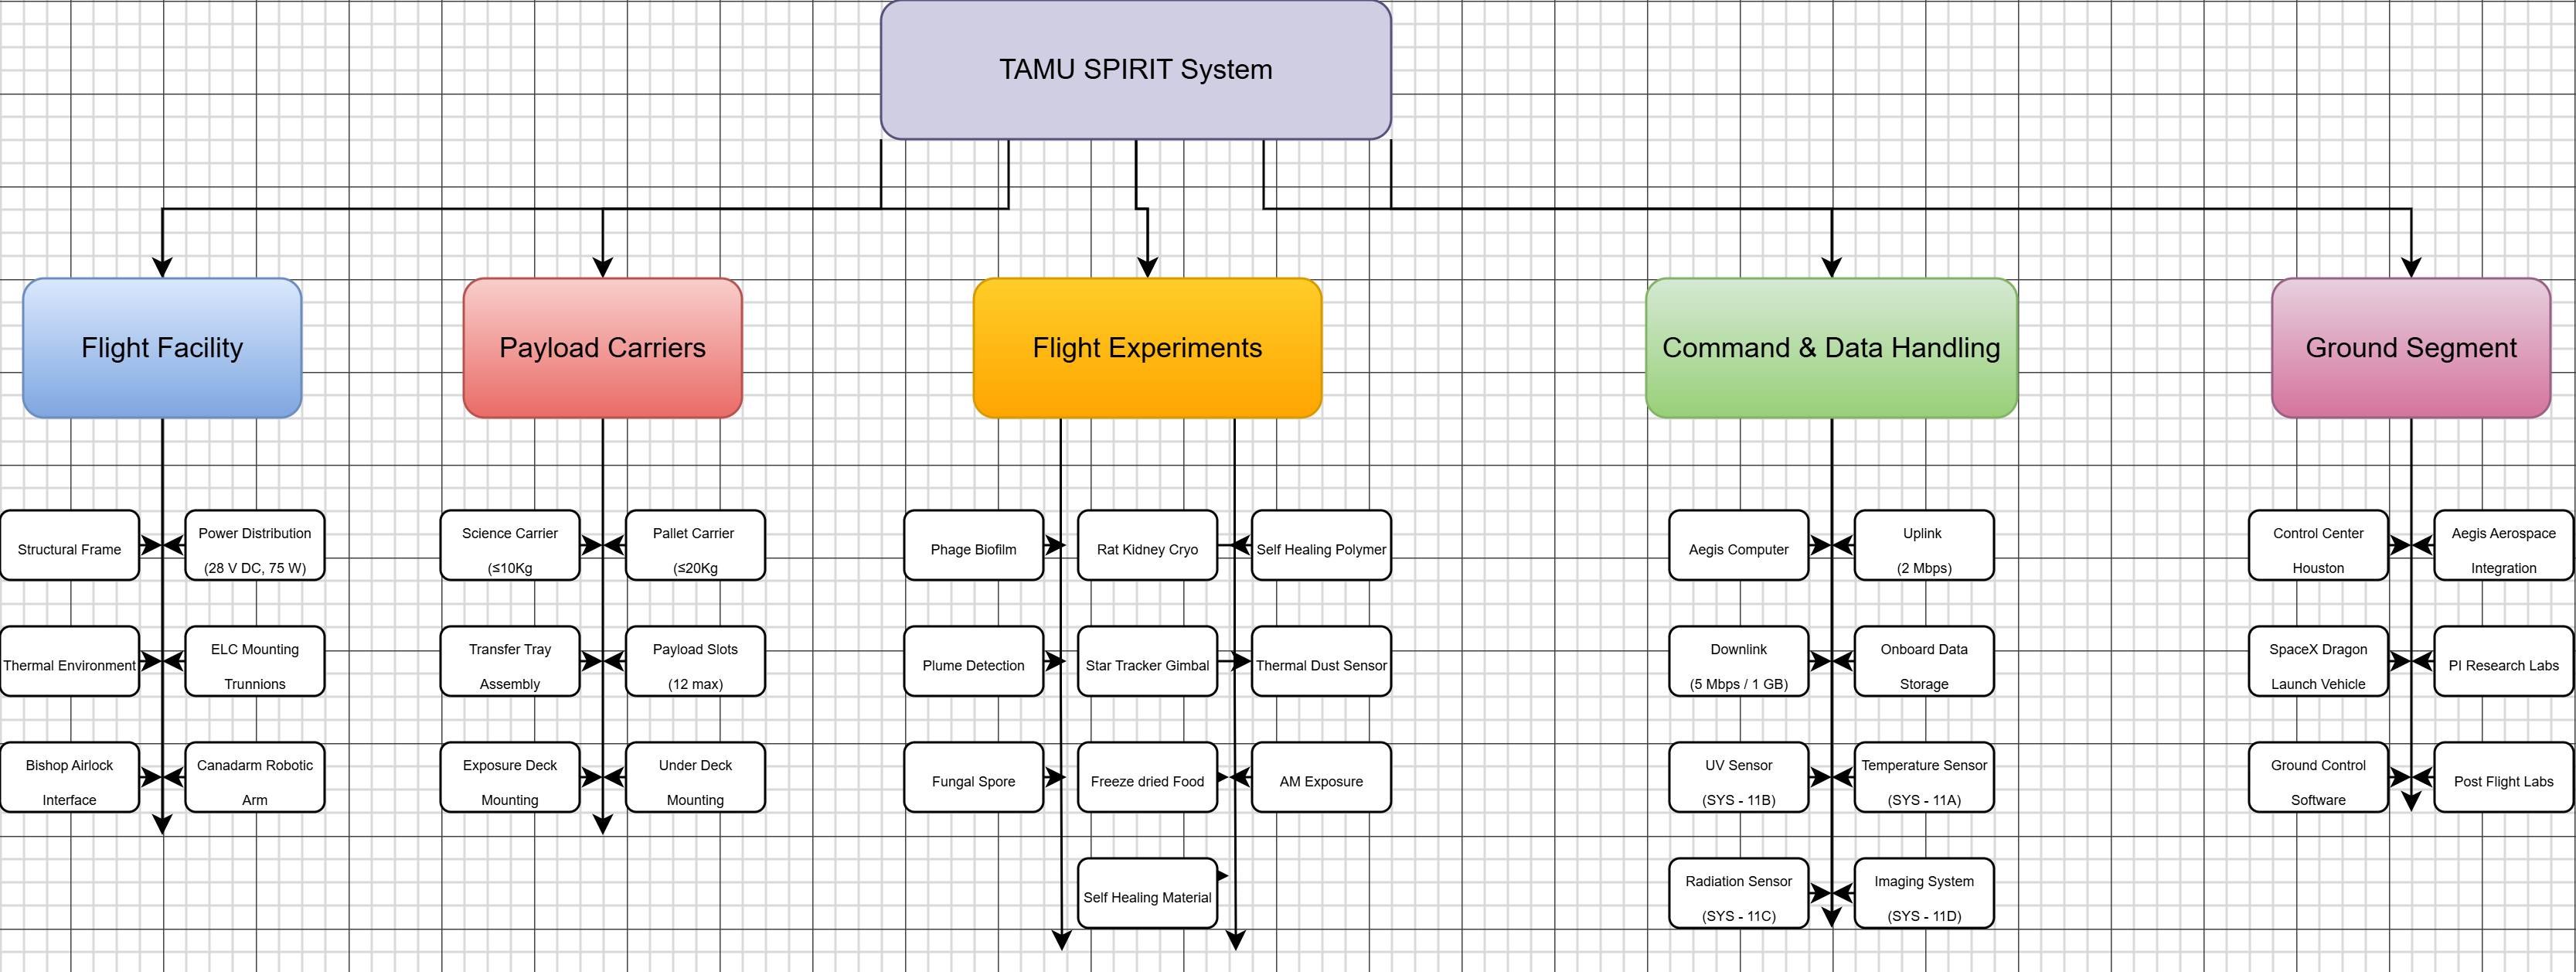
\includegraphics[width=\linewidth,height=0.78\textheight,keepaspectratio]{System_Decomp_Flowchart.drawio_1.png}
    \caption{System Decomposition Flowchart}
    \label{fig:system_decomp_flowchart}
\end{figure}

As a systems engineering mission, one of the most important aspects of developing technical solutions for this project is the system architecture that is followed for the total system, and the lower level sub-systems. The architecture of the system is the means by which a conceptual solution becomes a technical design. While the development of a system architecture is typically something that comes naturally, it's important to recognize what architecture is being used, why it's used, and how it is applied to sections of the systems.

The architecture that this project team uses is a synthesis-based architecture. By referencing previously designed architectures that were used by previous TAMU-SPIRIT teams, PI research groups, and the individual knowledge of the members, our team is able to modify what works and what does not for each subsystem with high resolution trade studies, creating an entirely new architecture supported by historical data. This, along with applying collective discussion, develops a bridge between the concepts and future design plans. This method works well since our primary mission has highly diverse subsystems, each with the potential to be its own high-level mission. So by referencing previously used architectures, and dissecting the primary elements from each one, the mission can be produced at a faster rate without sacrificing detail or refinement.

For each subsystem, a source of information was identified for each PI, identifying the needs, scope, and limitations of the desired experiment. Whether that be a PI research proposal, a previous TAMU-SPIRIT document, or a meeting with graduate students, this source is the keystone to the architecture. Research is then done on the results from previous tangible accomplishments in the field of interest, which is typically also provided by the PI or graduate student, but can also come from external and independent studies. Finally, the technical research is combined with the initial experiment goals, and creates an outline of general achievable objectives. By implementing high-level trade studies for the objective, a detailed bridge between conceptual goals and technical solutions can be established.

This process is iterated throughout all of the subsystems that were selected, and a system architecture is established. For the overall system, a web of interconnected architectures exists, where each can be independently developed, but each subsystem benefits from the advancement of another. This is exemplified when there are overlapping characteristics between subsystems, and the architecture web allows for a reduction of complexity by solving two issues simultaneously.

When the subsystem and full system architecture are developed, the mission operations are the next priority. One way to help break down a complex mission is through diagrams and visuals. Below is a visual of the Functional Flow Block Diagram for this mission, which helps define system relations and examine lower-level processes. Another is the System Decomposition Diagram, which breaks down the components of the mission as a whole, which helps define boundaries of what systems belong where, and simplifies the form-function relationship.

\begin{figure}[H]
    \centering
    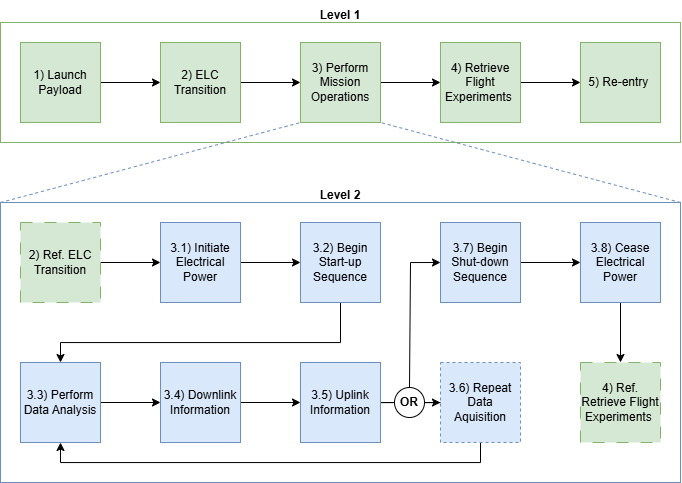
\includegraphics[width=\linewidth,height=0.78\textheight,keepaspectratio]{Functional_Flow_Block_Diagram.drawio.png}
    \caption{Functional Flow Block Diagram}
    \label{fig:functional_flow_block_diagram}
\end{figure}

\clearpage
\section{System Requirements}

The following system requirements define the functional, structural, and operational capabilities necessary for the TAMU-SPIRIT platform to support externally mounted flight experiments on the International Space Station (ISS) in Low Earth Orbit (LEO). These requirements are derived from stakeholder needs, system goals, and ISS interface constraints, and they ensure that hosted payloads can be safely integrated, powered, operated, and retrieved throughout the mission lifecycle. Overall, they establish the minimum performance, safety, and compatibility criteria required for TAMU-SPIRIT to enable long-duration exposure experiments and successful return of flight hardware for post-mission analysis. The following table, Table 2, outlines the highest level system requirements for the TAMU SPIRIT. Information regarding the traceability nomenclature can be found in Appendix A.

{\footnotesize
\setlength{\tabcolsep}{4pt}
\renewcommand{\arraystretch}{1.15}
\begin{longtable}{@{}p{2.2cm}p{4.1cm}p{4.1cm}p{4.1cm}@{}}
\caption{System Requirements}\label{tab:system_level_requirements}\\
\toprule
\textbf{Requirement ID and Traceability} & \textbf{Requirement} & \textbf{Rationale} & \textbf{Verification Method} \\
\midrule
\endfirsthead
\toprule
\textbf{Requirement ID and Traceability} & \textbf{Requirement} & \textbf{Rationale} & \textbf{Verification Method} \\
\midrule
\endhead
\bottomrule
\endfoot

SYS-1\\SN-T1, SN-T2, PG-1, SG-1, SG-2, SG-5 &
The TAMU-SPIRIT shall accommodate no fewer than 12 Science/Payload Carriers (SC/PC) simultaneously &
Supports multi-user missions and accessibility to long-duration research platforms. &
Inspection of carrier slot count in TAMU-SPIRIT flight hardware. \\

SYS-2\\SN-N2, SN-A1, SN-SX1, SG-1, SG-3, SG-4 &
The TAMU-SPIRIT system shall provide standardized mechanical mounting interfaces for all integrated SC/PC payloads. &
Ensures experiments have secure attachment, power, and data access. &
Inspection of interface drawings and hardware configuration. \\

SYS-3\\SN-T2, SN-A1, SG-1, SG-2, SG-3 &
The TAMU-SPIRIT system shall provide standardized electrical power and data interfaces to each integrated SC/PC payload. &
Maximizes flexibility in research objectives and improves efficiency in time, cost, and mass. &
Interface inspection and functional test of power/data connections. \\

SYS-4\\SN-T1, SN-T2, SG-2, SG-3, SG-4, SG-5 &
TAMU-SPIRIT shall provide a minimum uplink and downlink data capacity of 1 GB per week per payload. &
Enables experiment-related data transfer to the ground. &
End-to-end communication demonstration with Payload Operations Control Center (POCC). \\

SYS-5A\\SN-N1, SN-N2, SN-A1, SN-SX1, SG-3, SG-4 &
All integrated SC and PC payloads shall pass vibration testing consistent with launch vehicle requirements. &
Ensures mission success and mitigates hazards to crew, experiments, TAMU-SPIRIT, and ISS. &
Vibration test report. \\

SYS-5B\\SN-N1, SN-A1, SG-3, SG-4 &
All integrated SC and PC Payloads shall pass thermal cycling consistent with ISS operational conditions. &
 &
Thermal cycling test report. \\

SYS-5C\\SN-N1, SN-N2, SN-N3, SN-U1, SG-1, SG-4 &
All integrated SC and PC payloads shall obtain NASA safety approval prior to launch. &
 &
Documentation review and certification record. \\

SYS-6\\PG-2, SG-2, SG-4, SG-5 &
TAMU-SPIRIT shall support continuous payload operation for a minimum of 6 months and up to 12 months per deployment cycle. &
Enables long-term research aligned with ISS timelines. &
Analysis of power, thermal, and operational lifetime. \\

SYS-7\\SN-N2, SN-SX1, SG-1, SG-4 &
TAMU-SPIRIT shall interface with ISS-compatible cargo transport vehicles. &
Enables successful transportation to the ISS. &
Interface compatibility documentation review. \\

SYS-8\\SN-N5, SG-1, SG-4 &
TAMU-SPIRIT shall allow retrieval of SCs/PCs using the ISS robotic arm via the Transfer Tray. &
Ensures safe, controlled, and automated experiment handling. &
Demonstration and interface compliance review. \\

SYS-9\\SN-A1, SN-SX1, PG-3, SG-4, SG-5 &
TAMU-SPIRIT shall support standardized procedures for integration, de-integration, and packaging for return to Earth. &
Ensures safe, repeatable handling and successful hardware retrieval. &
Testing of standardized procedures and inspection throughout the process. \\

SYS-10\\SN-N5, SN-T2, SG-2, SG-3, SG-4 &
TAMU-SPIRIT shall enable ground-based command and control via the POCC. &
Enables ground-based command while minimizing ISS crew involvement. &
Communications test with POCC. \\

SYS-11A\\SN-T1, SN-PI2, SG-2, SG-4, SG-5 &
TAMU-SPIRIT shall provide temperature data for exposed-deck carriers. &
Environmental data is required to correlate observed changes in material or sensor performance with actual on-orbit exposure conditions. &
Sensor calibration and functional test. \\

SYS-11B\\SN-T1, SN-PI2, SG-2, SG-4, SG-5 &
TAMU-SPIRIT shall provide ultraviolet exposure data for exposed deck carriers. &
 &
Sensor calibration and validation. \\

SYS-11C\\SN-T1, SN-PI2, SG-2, SG-4, SG-5 &
TAMU-SPIRIT shall provide ionizing radiation exposure data for exposed deck carriers. &
 &
Dosimeter calibration and validation. \\

SYS-11D\\SN-T1, SN-PI2, SG-2, SG-4, SG-5 &
TAMU-SPIRIT shall provide visual imagery of exposed deck carriers. &
 &
Functional camera testing. \\
\end{longtable}
}

The following tables, Table 3 and Table 4, disclose the requirements specific to the pallet carriers (PC) and the science carriers (SC), respectively, as outlined in the TAMU-SPIRIT Quick Reference Guide [2].

\begin{table}[!htbp]
    \centering
    \footnotesize
    \setlength{\tabcolsep}{4pt}
    \renewcommand{\arraystretch}{1.15}
    \begin{tabularx}{\textwidth}{@{}>{\raggedright\arraybackslash}p{2.2cm}YYY@{}}
    \toprule
    \textbf{Requirement ID and Traceability} & \textbf{Requirement} & \textbf{Rationale} & \textbf{Verification Method} \\
    \midrule
    PC-SYS-1\\SN-T2, SN-SX1, SG-1, SG-3, SG-4 &
    The TAMU-SPIRIT system shall accommodate PC payloads with external dimensions not exceeding: 42.16 cm $\times$ 21.84 cm $\times$ 25.07 cm (L $\times$ W $\times$ H) &
    Ensures experiment compatibility with carrier dimensions. &
    Pre-flight integration dimensional inspection. \\

    PC-SYS-2\\SN-T2, SG-2, SG-3 &
    TAMU-SPIRIT shall provide 60 W of electrical power to each PC payload. &
    Provides sufficient power for larger active experiments. &
    Ground functional power test. \\

    PC-SYS-3\\SN-N2, SN-SX1, SN-U1, SG-3, SG-4 &
    PC Payload mass shall not exceed 20 kg. &
    Mitigates launch and integration risk through mass limitation. &
    Weighing of each PC prior to integration. \\
    \bottomrule
    \end{tabularx}
    \caption{Pallet Carrier Requirements}
    \label{tab:pc_requirements}
\end{table}

\begin{table}[!htbp]
    \centering
    \footnotesize
    \setlength{\tabcolsep}{4pt}
    \renewcommand{\arraystretch}{1.15}
    \begin{tabularx}{\textwidth}{@{}>{\raggedright\arraybackslash}p{2.2cm}YYY@{}}
    \toprule
    \textbf{Requirement ID and Traceability} & \textbf{Requirement} & \textbf{Rationale} & \textbf{Verification Method} \\
    \midrule
    SC-SYS-1\\SN-N2, SN-SX1, SN-U1, SG-3, SG-4 &
    SC payload mass shall not exceed 8 kg. &
    Mitigates launch and integration risk through mass limitation. &
    Weighing of each SC prior to integration. \\

    SC-SYS-2\\SN-T2, SG-2, SG-3 &
    TAMU-SPIRIT shall supply 50 W of electrical power to each SC payload. &
    Provides sufficient power for active experiments. &
    Ground functional power test. \\

    SC-SYS-3\\SN-T2, SN-SX1, SG-1, SG-3, SG-4 &
    TAMU-SPIRIT SCs shall fit within volume constraints: 24.05 cm $\times$ 18.03 cm $\times$ 0.64 cm (Exposure Deck Mounting) and 31.24 cm $\times$ 17.78 cm $\times$ 7.94 cm (Under Deck Mounting). &
    Ensures experiment compatibility with carrier dimensions. &
    Pre-flight dimensional measurement and inspection within SC. \\
    \bottomrule
    \end{tabularx}
    \caption{Science Carrier Requirements}
    \label{tab:sc_requirements}
\end{table}

\clearpage
\section{Subsystem Requirements}

This section defines subsystem-level requirements for each candidate flight experiment. Requirement wording, rationale, and verification methods were converted from the SRR source material into a consistent LaTeX format. The scope includes ten experiments aligned to current TAMU-SPIRIT candidate activities.

\subsection{1. Thermal Dust Sensor Exposure}

The Thermal Dust Sensor Exposure experiment (TDS) is an active flight experiment that has passed initial downselection. The experiment involves direct exposure of a thermal sensor - initially designed to be used to sense a layer of dust on a lunar or martian surface - to understand the behavior of thermal sensors when exposed to solar radiation and a deep space environment. The project team's mission is to modify the existing sensor apparatus to measure the degradation due to long-term radiation. The primary stakeholders and PI, Dr. Richard Kurwitz, will provide the pre-designed sensor for the system team to make it compatible with the Aegis experiment carriers. Therefore, the goals for this experiment are the following:

\vspace{0.3em}
\begin{enumerate}[leftmargin=*]
    \item Measure thermal values used to estimate changes in the emissivity of the device in orbit as a baseline condition of the sensor (TDS-G1).
    \item Compare the device against the control data set to quantify the calculations of radiative degradation due to the orbital environment (TDS-G2).
\end{enumerate}

The requirements for this experiment are shown in Table~\ref{tab:tds_requirements} which were developed with the assistance of a research proposal document for the lunar dust sensor.

\begin{table}[H]
    \centering
    \footnotesize
    \setlength{\tabcolsep}{4pt}
    \renewcommand{\arraystretch}{1.15}
    \begin{tabularx}{\textwidth}{@{}>{\raggedright\arraybackslash}p{2.4cm}YYY@{}}
    \toprule
    \textbf{Requirement ID and Traceability} & \textbf{Requirement} & \textbf{Rationale} & \textbf{Verification Method} \\
    \midrule
    TDS-R1\\TDS-G1 &
    The experiment shall quantify the degradation of the sensor through control test comparison and calculations. &
    The sensor must be able to observe any potential dust and quantify thermal energy balance to determine quantity of dust. &
    Control tests will be performed using dust on earth to ensure proper calibration. \\

    TDS-R2\\TDS-G1 &
    The experiment shall be oriented to minimize parasitic thermal radiation from the ISS.. &
    The experiment must isolate the effects of the space environment on the sensor to provide more accurate conclusions. &
    A number of tests on the impacts of parasitic thermal radiation will be performed, and proper orientation will be developed. \\

    TDS-R3\\SYS-4 &
    The experiment shall return data within a 1 GB daily maximum downlink. &
    The experiment must not exceed daily downlink bandwidth. &
    Testing of the maximum required bandwidth of data will take place. \\

    TDS-R4\\PC-SYS-2 &
    The experiment shall consume no more than a maximum of 60W when operational, and 30W when non-operational. &
    The experiment must remain within power limits allocated to the carrier. &
    The power needs of the sensor will be calculated and tested. \\

    TDS-R5\\TDS-G2 &
    The experiment shall estimate emissivity at a rate of no less than once every 3-6 days over the course of 6-12 months. &
    The lifespan of the experiment must extend to entirety of the mission to remain significant for research &
    Multiple tests and calculations will take place to ensure the longevity of the sensor. \\
    \bottomrule
    \end{tabularx}
    \caption{TDS Requirements}
    \label{tab:tds_requirements}
\end{table}


\clearpage
\subsection{2. Micro-Gravity Vortex Separator}

The Micro-Gravity Vortex Separator experiment (MGVS) is part of a cutting-edge research operation that aims to form a gravity-independent Rankine cycle with the use of vortex phase separators. These phase separators allow for stable nucleate boiling and efficient direct-contact condensation that can be used in micro-gravity, unlike buoyancy driven separation. Break-through in this field has an opportunity to allow for a high-efficiency, lightweight power source, viable for long-term, deep space missions. The PI, Dr. Richard Kurwitz, and his research group will work with the system team to assist in the development of this experiment as a starting point for further research. The goals of this experiment are the following:

\vspace{0.3em}
\begin{enumerate}[leftmargin=*]
    \item Fabricate and characterize the key components of a vortex boiler/condenser such that a Rankine cycle can be performed in micro-gravity (MGVS-G1).
    \item Reinforce experimentally derived models with ground-test data and validate performance of vortex systems. (MGVS-G2).
\end{enumerate}

The requirements shown in Table~\ref{tab:mgvs_requirements} outline the requirements that have been formulated with the help of Dr. Kurwitz, and the specific aims he had selected for the timeline of the research project.

\begin{table}[H]
    \centering
    \footnotesize
    \setlength{\tabcolsep}{4pt}
    \renewcommand{\arraystretch}{1.15}
    \begin{tabularx}{\textwidth}{@{}>{\raggedright\arraybackslash}p{2.4cm}YYY@{}}
    \toprule
    \textbf{Requirement ID and Traceability} & \textbf{Requirement} & \textbf{Rationale} & \textbf{Verification Method} \\
    \midrule
    MGVS-R1\\SYS-4 &
    Vortex-condenser operating two-phase flow shall return flow dynamic properties within 1 GB/weekday downlink. &
    Data coming from the vortex-condenser must be returned for model refining. &
    The bandwidth requirement of thermodynamic sensors shall be tested. \\

    MGVS-R2\\MGVS-G1 &
    Vortex-boiler shall return modeling data at a refinement such that further discretization yields <5\% variation &
    The experiment must reach this degree of refinement to allow for the most accurate modeling of vapor core and liquid replenishment. &
    Various refinement levels will be tested to calculate the 5\% deviation mesh. \\

    MGVS-R3\\PC-SYS-2 &
    Vortex heat exchangers shall consume a maximum of 30W each at 28V DC. &
    The combination of heat exchangers must not exceed maximum power provided. &
    The power needs of the heat exchangers will be calculated and experimentally tested. \\

    MGVS-R4\\MVGS-G1 &
    Vortex-condenser heat transfer correlation shall be refined with ground-test data during flight. &
    The condenser must use ground-data to observe the impacts of micro-gravity and improve estimates of heat transfer correlations. &
    Analysis on sample data will ensure that refinement methods for this experiment are available and physically appropriate. \\

    MGVS-R5\\MGVS-G2 &
    Generation of reduced-order boiling models shall return critical heat flux and superheat values in a variety of differing flow swirls. &
    The developed model must account for a variety of different conditions and fluids. &
    Iterative testing of ground-test vortex separators in differing conditions will ensure accurate modelling. \\
    \bottomrule
    \end{tabularx}
    \caption{MGVS Requirements}
    \label{tab:mgvs_requirements}
\end{table}


\clearpage
\subsection{3. Cryogenic Preservation of Mammalian Organs}

The objective of the experiment is to design a space-compliant cryogenic system to preserve vitrified mammalian organs for at least six months before returning to earth for transplantation into recipient specimens. There are two primary goals for this flight experiment. The first is to ensure that the chamber(s) designed for the experiment are structurally resilient to the pressure experienced throughout all mission stages and maintain a leak-proof internally isochoric environment entirely autonomously under the TAMU-SPIRIT resource constraints (CPMO-G1). The second goal is to maintain physical containment of all specimens and to ensure that each kidney stays in a vitrified state for the full on-orbit mission (CPMO-G2). The requirements shown below in Table~\ref{tab:cpmo_requirements} include information collected in collaboration with the current AERO 402 group responsible for this experiment.

\vspace{0.3em}
\begin{enumerate}[leftmargin=*]
    \item Ensure that the chamber(s) designed for the experiment are structurally resilient to the pressure experienced throughout all mission stages and maintain a leak-proof internally isochoric environment entirely autonomously under the TAMU-SPIRIT resource constraints (CPMO-G1).
    \item Maintain physical containment of all specimens and ensure that each kidney stays in a vitrified state for the full on-orbit mission (CPMO-G2).
\end{enumerate}

\begin{table}[H]
    \centering
    \footnotesize
    \setlength{\tabcolsep}{4pt}
    \renewcommand{\arraystretch}{1.15}
    \begin{tabularx}{\textwidth}{@{}>{\raggedright\arraybackslash}p{2.4cm}YYY@{}}
    \toprule
    \textbf{Requirement ID and Traceability} & \textbf{Requirement} & \textbf{Rationale} & \textbf{Verification Method} \\
    \midrule
    CPMO-R1\\CPMO-G2 &
    The flight experiment shall maintain the mammalian kidneys at roughly -100℃ from the time of extraction, through the full mission, to the time of transplantation. &
    The rodent kidneys need to maintain a vitrified state without forming ice crystals but at a temperature consistent with long term cryogenic storage. &
    The internal temperature of the flight experiment chamber(s) will be continuously logged through the mission. The temperature of each specimen will be collected before and after the mission. \\

    CPMO-R2\\CPMO-G1 &
    The flight experiment chamber shall structurally withstand the pressure experienced during the flight without deformation of the chamber or specimen. &
    Proper structural integrity of the flight experiment chamber(s) must be upheld to prevent mechanical damage to the specimens that could hinder transplantation. &
    Finite Element Analysis (FEA) will be used on all prototyped chamber systems, to ensure they can withstand a 20G expected load (10G maximum force with Factor of Safety = 2). \\

    CPMO-R3\\CPMO-G2 &
    The flight subchambers shall uphold physical separation between the individual specimens. &
    Each specimen must be independently contained to prevent shared failure modes or cross contamination that could compromise transplantation viability. &
    A triple-walled cooling system will individually surround each kidney. The subchambers will be dye tested during prototyping to ensure there is no transfer between cavities. \\

    CPMO-R4\\CPMO-G1 &
    The flight experiment shall maintain a leak-proof seal with constant volume for the entire mission duration. &
    This flight experiment poses a high environmental risk, and maintaining an internally isochoric environment will prevent the release of biological matter to the surroundings. &
    The internal pressure of the flight experiment chamber(s) will be continuously logged through the mission. The chamber(s) will be dye tested during prototyping to ensure there is no change in volume. \\

    CPMO-R5\\CPMO-G1 &
    The flight experiment shall operate entirely autonomously within the mass, volume, and power constraints of the carrier. &
    Ensures that the flight experiment is compliant with all TAMU-SPIRIT equipment and power constraints. &
    Mass, volume, and power data will be both simulated and verified before launch on an integrated test platform. \\

    CPMO-R6\\CPMO-G1 &
    The flight experiment shall operate autonomously without carrier supplied power for at least 72 hours. &
    This is a conservative estimate of the time that the flight experiment will be without access to the SPIRIT power source. This ensures that the specimens will sustain their vitrified state during transition to the vehicle. &
    Thermal simulations will be conducted. Ground testing of the flight experiment in a fully integrated carrier, with the thermal and pressure sensors active, and the heating rate of the cooling system being measured. \\
    \bottomrule
    \end{tabularx}
    \caption{CPMO Requirements}
    \label{tab:cpmo_requirements}
\end{table}


\clearpage
\subsection{4. Autonomous Classification and Tracking of Plumes}

Autonomous Classification and Tracking of Plumes (ACT-P) maintains the scientific objective of the acquisition of high spatiotemporal fidelity imagery of atmospheric plume events via active sensing to improve training sets for detection of rare plume events on the Lunar surface. ACT-P has launched several balloon-based high-altitude imaging systems to image the Earth's surface with mixed results. The ACT-P team working under Dr. Daniel Selva's System Engineering, Autonomy, and Knowledge (SEAK) lab maintains that a space-based system aboard TAMU-SPIRIT would improve the likelihood of plume event detection as well as the operational lifespan of the system. Therefore, the primary goals of the flight experiment are as follows:

\vspace{0.3em}
\begin{enumerate}[leftmargin=*]
    \item Acquire high spatiotemporal fidelity of plume-relevant imagery on-orbit using autonomous gimbaled acquisition and deliver a machine-learning (ML) ready dataset to ground teams for improving current generation detection models (ACTP-G1).
    \item Enable a safe update-and-test loop where a ground-trained updated model can be deployed and compared against the baseline model on-orbit under controlled conditions producing quantitative performance evidence (ACTP-G2).
\end{enumerate}

The requirements for this experiment are shown in Table~\ref{tab:actp_requirements}.

\begin{table}[H]
    \centering
    \footnotesize
    \setlength{\tabcolsep}{4pt}
    \renewcommand{\arraystretch}{1.15}
    \begin{tabularx}{\textwidth}{@{}>{\raggedright\arraybackslash}p{2.4cm}YYY@{}}
    \toprule
    \textbf{Requirement ID and Traceability} & \textbf{Requirement} & \textbf{Rationale} & \textbf{Verification Method} \\
    \midrule
    ACTP-R1\\ACTP-G1 &
    The flight experiment shall autonomously direct pointing/acquisition behavior using an on-board pretrained plume detection capability &
    Autonomous pointing and data collection aid in the increased temporal fidelity of the dataset &
    Testing of the full system against a digitally simulated orbit \\

    ACTP-R2\\ACTP-G1 &
    The flight experiment shall ensure bounded and stable pointing behavior during autonomous operations with fault detection &
    Gimbal fault detection and unstable pointing behavior represented critical failures in past tests and similar events would result in mission failure &
    Red-teaming / antagonistic testing of gimbal control authority \\

    ACTP-R3\\ACTP-G1 &
    The flight experiment shall produce and time-align acquisition metadata sufficient for downstream ML reuse and reconstruction &
    Recreating of on-orbit conditions enables the training and quantitative comparison of improved ML models &
    Inspection of system's output which contains all parameters required for training \\

    ACTP-R4\\ACTP-G1 &
    The flight experiment shall preserve dataset integrity and provenance from acquisition through delivery to ground teams using verifiable completeness and corruption detection &
    Prevent corruption or mislabeling of imagery and metadata collected from the system to ensure reproducibility &
    Red-teaming / antagonistic testing of data store and/or transmission systems \\

    ACTP-R5\\ACTP-G1 &
    The flight experiment shall support routine operations with weekly monitoring by providing health telemetry, general fault observability, and recoverability &
    Prevent critical, cascading failures and enable return to a safe state &
    Red-teaming / antagonistic testing of critical fault recovery subsystems. \\

    ACTP-R6\\ACTP-G2 &
    The flight experiment should support deployment of ground-trained updated models to the flight system with a controlled lifecycle &
    Enable verification of primary mission objective to improve dataset quality and consequently model performance &
    Simulated on-orbit update of model without critical, unrecoverable faults \\
    \bottomrule
    \end{tabularx}
    \caption{ACTP Requirements}
    \label{tab:actp_requirements}
\end{table}


\clearpage
\subsection{5. Spaceflight Resilience of Food Fermentation Fungi}

The scientific objective of this flight experiment is to evaluate the viability of food-relevant fungal spores following exposure to a spaceflight environment. The spores of A. oryzae, R. oryzae, R. microsporus, and N. intermedia will be produced under standardized laboratory conditions, harvested, desiccated to a specified moisture content, and sealed in their respective containers. The three high-level goals of this experiment is to assess the viability of all four spore samples following a six-month exposure flight (SRFFF-G1), to compare the viability, germination rate, and growth kinetics of space-exposed spores with Earth-based ground control spores (SRFFF-G2), and to assess the effects of space-exposure on the fermentation performance, metabolite production capacity, and safety of the recovered fungal strains (SRFFF-G3). The hypothesized outcome is that the experimental spores will remain viable all the while exhibiting subtle molecular and metabolic adaptations to microgravity and space radiation. Dr. Reza Ovissipour and his research team will be advising the flight experiment. Below are the outlined requirements developed to achieve these flight experiment goals.

\begin{table}[H]
    \centering
    \footnotesize
    \setlength{\tabcolsep}{4pt}
    \renewcommand{\arraystretch}{1.15}
    \begin{tabularx}{\textwidth}{@{}>{\raggedright\arraybackslash}p{2.4cm}YYY@{}}
    \toprule
    \textbf{Requirement ID and Traceability} & \textbf{Requirement} & \textbf{Rationale} & \textbf{Verification Method} \\
    \midrule
    SRFFF-R1\\SRFFF-G2, SRFFF-G3 &
    The flight experiment shall host the harvested spores, desiccated to a moisture content of 10\%, within hermetically sealed containers that prevent microbial contamination. &
    Ensures that no foreign microbes permeate the spore samples, maintaining the integrity, accuracy, and viability of research efforts. &
    Laboratory moisture analysis will confirm that spores are desiccated to 10\%, containers will be subjected to leak tests, and sterility assessment will be performed prior to sealing the samples. \\

    SRFFF-R2\\SRFFF-G2, SRFFF-G3 &
    The flight experiment shall expose the spore samples to a total ionizing dose within $\pm$10\% of the externally measured radiation environment. &
    Crucial for post-flight comparisons to ground control spore samples. &
    Install passive or active radiation dosimeters adjacent to the spore samples. \\

    SRFFF-R3\\SRFFF-G1 &
    The flight experiment shall measure and record the temperature and radiation dose experienced by the spore samples throughout the 6 month flight duration. &
    Recorded and retrieved data will aid in correlating the observed sample changes to the environmental conditions they were exposed to. &
    Install temperature and radiation sensors that track and record experiment exposure data for the entirety of the flight duration. \\

    SRFFF-R4\\SRFFF-G1 &
    The flight experiment chamber shall structurally secure the four spore samples and withstand the mechanical and thermal loading inherent to launch and reentry operations. &
    Ensures that the sample containers maintain their structural integrity and placement under loading. &
    Structural analysis, vibration testing, and hardware mounting will be conducted and assessed prior to launching. \\

    SRFFF-R5\\SRFFF-G2 &
    The flight experiment shall enable the safe removal of all four spore sample containers from the carrier upon its return to Earth. &
    Satisfies the primary objective of the flight experiment to compare space-exposed spore samples to Earth-based control samples. &
    A ground operations test will be conducted to evaluate the removal procedures of the sample containers, and hardware configuration will be assessed for accessibility. \\
    \bottomrule
    \end{tabularx}
    \caption{SRFFF Requirements}
    \label{tab:srfff_requirements}
\end{table}


\clearpage
\subsection{6. Freeze-Dried Food Analogs}

The scientific objective of this flight experiment is to assess the suitability of meat alternatives for space missions by measuring lipid oxidation as a proxy for product quality. The intent would be to expose up to four freeze-dried food samples, ranging from cultivated meat to plant-based meat alternatives, to a spaceflight environment. The three high-level goals of this experiment is to compare the viability of space-exposed freeze-dried food samples with Earth-based ground control samples (FDFA-G1), to perform Thiobarbituric Acid Reactive Substances (TBARS) assays for post-flight analysis (FDFA-G2), and to quantify the effects of long-duration radiation exposure on the structural and nutritional integrity of the freeze-dried food samples (FDFA-G3). Dr. Reza Ovissipour and his research team will be advising the flight experiment. Below are the outlined requirements developed to achieve these flight experiment goals.

\begin{table}[H]
    \centering
    \footnotesize
    \setlength{\tabcolsep}{4pt}
    \renewcommand{\arraystretch}{1.15}
    \begin{tabularx}{\textwidth}{@{}>{\raggedright\arraybackslash}p{2.4cm}YYY@{}}
    \toprule
    \textbf{Requirement ID and Traceability} & \textbf{Requirement} & \textbf{Rationale} & \textbf{Verification Method} \\
    \midrule
    FDFA-R1\\FDFA-G1, FDFA-G3 &
    The flight experiment shall expose the freeze-dried food samples to the outer space environment for a flight duration of 6 months. &
    Crucial for post-flight research methodology and comparisons to ground control food samples. &
    Install passive or active radiation dosimeters adjacent to the freeze-dried food samples. \\

    FDFA-R2\\FDFA-G2, FDFA-G3 &
    The flight experiment shall seal the samples in sterile, contamination-proof containers that prevent moisture infiltration. &
    Ensures that there is no sample degradation or microbial growth, maintaining the integrity, accuracy, and viability of research efforts. &
    Sample containers will be subjected to leak tests, and sterility assessment will be performed prior to sealing the samples. \\

    FDFA-R3\\FDFA-G3 &
    The flight experiment shall measure and record the temperature and radiation dose experienced by the freeze-dried food samples throughout the entire flight duration. &
    Recorded and retrieved data will aid in correlating the observed sample changes to the environmental conditions they were exposed to. &
    Install temperature and radiation sensors that track and record experiment exposure data for the entirety of the flight duration. \\

    FDFA-R4\\FDFA-G1, FDFA-G2 &
    The flight experiment chamber shall protect and secure all samples from mechanical and thermal loads experienced during launch and reentry operations. &
    Ensures that the sample containers maintain their structural integrity and placement under loading. &
    Structural analysis, vibration testing, and hardware mounting will be conducted and assessed prior to launching. \\

    FDFA-R5\\FDFA-G1 &
    The flight experiment shall enable the safe removal of all four spore sample containers from the carrier upon its return to Earth. &
    Satisfies the primary objective of the flight experiment to compare space-exposed freeze-dried food samples to Earth-based control samples. &
    A ground operations test will be conducted to evaluate the removal procedures of the sample containers, and hardware configuration will be assessed for accessibility. \\

    FDFA-R6\\FDFA-G2 &
    The flight experiment shall accommodate a mass of 5-10 grams for each sample, with a possibility of sending up to four samples. &
    Ensures that there is enough sample to perform TBARS assays for post-flight analysis. &
    Individually assess the mass of each sample and compare against the carrier's mass and volume constraints. \\
    \bottomrule
    \end{tabularx}
    \caption{FDFA Requirements}
    \label{tab:fdfa_requirements}
\end{table}


\clearpage
\subsection{7. Dials-Alder Based Self-Healing Exposure (DASH)}

The scientific objective of this flight experiment is to determine whether Diels-Alder self-healing polymers - materials capable of autonomously repairing cracks at the molecular level by reforming broken chemical bonds - retain that healing ability after prolonged exposure to the space environment. Two goals of this experiment are to assess the self-healing capabilities of Diels-Alder Polymer (DAP) samples following environmental exposure to space, by comparing the tensile strength and material properties of flight samples against ground-controlled samples that experienced no space exposure (DASH-G1). The second goal aims to determine how thermal cycling and cosmic irradiation individually and collectively affect DAP sample degradation and influence the sample's self-healing performance, which will be achieved through the separation of samples into three experimental groups, each subjected to a different environment (DASH-G2). Together, these goals will determine whether DAP is a viable material to be used for space applications. Outlined in Table [placeholder] are the requirements established to achieve these goals.

\vspace{0.3em}
\begin{enumerate}[leftmargin=*]
    \item Assess the self-healing capabilities of Diels-Alder Polymer (DAP) samples following environmental exposure to space, by comparing the tensile strength and material properties of flight samples against ground-controlled samples that experienced no space exposure (DASH-G1).
    \item Determine how thermal cycling and cosmic irradiation individually and collectively affect DAP sample degradation and influence the sample's self-healing performance, which will be achieved through the separation of samples into three experimental groups, each subjected to a different environment (DASH-G2).
\end{enumerate}

\begin{table}[H]
    \centering
    \footnotesize
    \setlength{\tabcolsep}{4pt}
    \renewcommand{\arraystretch}{1.15}
    \begin{tabularx}{\textwidth}{@{}>{\raggedright\arraybackslash}p{2.4cm}YYY@{}}
    \toprule
    \textbf{Requirement ID and Traceability} & \textbf{Requirement} & \textbf{Rationale} & \textbf{Verification Method} \\
    \midrule
    DASH-R1\\DASH-G1, DASH-G2 &
    The flight experiment shall accommodate nine samples of dimensions 30mm x 30mm x 0.5mm and a total mass of less than 9 grams. &
    The mass and volume constraint are derived from SC and PC's mass and volume budget and taking into account other flight experiments. &
    Measure all nine samples using calipers to confirm the volume constraint and weigh all nine samples together to confirm a total mass of less than 9 grams. \\

    DASH-R2\\DASH-G1, DASH-G2 &
    The flight experiment shall allow retrieval of all nine samples at the end of the mission for post flight analysis against ground samples. &
    Post flight analysis of returned samples against ground control samples is the primary scientific objective of this flight experiment. &
    Confirm all nine samples are retrieved upon the completion of the mission. \\

    DASH-R3\\DASH-G2 &
    The flight experiment shall ensure that Group 1 (Thermal Cycling) and Group 3 (Full Exposure) samples' temperature exposure is within a range of -100 °C to +100 °C throughout the mission duration. &
    The bounds of -100 °C to +100 °C reflect the upper and lower temperature limit the sample can handle without being damaged. &
    Implement a thermal sensor to ensure the temperature range the samples experience in Group 1 and Group 3 are within the range of 100 °C to +100 °C. \\

    DASH-R4\\DASH-G2 &
    The flight experiment shall ensure that Group 2 (Cosmic Irradiation) samples' temperature exposure is within a range of 0 °C to 30 °C. &
    Group 2 transition temperature is 0  °C to 30 °C, outside of this temperature range the sample can experience effects of chain stiffness. &
    Implement a thermal sensor to ensure the temperature range the samples experience in Group 2 is within the range of 0 °C to 30 °C. \\

    DASH-R5\\DASH-G1, DASH-G2 &
    The flight experiment shall record temperature and radiation exposure data for all three sample groups, with data retrieved post flight upon sample return to Earth. &
    Recorded data will help correlate observed sample changes with actual experienced conditions. &
    Implement temperature and radiation sensors to measure and record data over the duration of the mission. \\

    DASH-R6\\DASH-G2 &
    The flight experiment shall shield Group 1 (Thermal Cycling) samples from cosmic radiation for the duration of the mission. &
    Group 1 is a controlled experiment designed to only experience thermal cycling,  when contaminated with radiation it destroys the ability to attribute changes to thermal cycling alone. &
    Radiation testing of shielding material and thickness analysis pre-launch to minimize radiation leakage. \\
    \bottomrule
    \end{tabularx}
    \caption{DASH Requirements}
    \label{tab:dash_requirements}
\end{table}


\clearpage
\subsection{8. Event-Based Space Telescope (EBST)}

The objective of the Event-Based Space Telescope experiment is to validate a high angular-rate event-based star tracker and assess its attitude estimation performance under simulated tumbling and stationary conditions. This is particularly useful for ``lost in space'' scenarios in which a satellite finds itself unable to compute its attitude, needed to correct errant motion. The EBST seeks to solve this issue using a special event-based camera and proprietary estimation algorithm that significantly extends attitude estimation capability into higher angular rates. In order to achieve this, three high level goals are defined such that adequate conclusions can be obtained about the tracker and algorithm's effectiveness. The first is to simulate ``lost in space'' conditions by exposing the EBST to high angular rates in LEO (EBST-G1). The second goal is to perform onboard attitude estimation using data collected by the EBST using the proprietary algorithm (EBST-G2). Finally, the experiment will downlink all data necessary to quantitatively assess the effectiveness of the EBST and the attitude estimation algorithm (EBST-G3). Outlined below are the requirements needed to achieve these goals.

\vspace{0.3em}
\begin{enumerate}[leftmargin=*]
    \item Simulate ``lost in space'' conditions by exposing the EBST to high angular rates in LEO (EBST-G1).
    \item Perform onboard attitude estimation using data collected by the EBST using the proprietary algorithm (EBST-G2).
    \item Downlink all data necessary to quantitatively assess the effectiveness of the EBST and the attitude estimation algorithm (EBST-G3).
\end{enumerate}

\begin{table}[H]
    \centering
    \footnotesize
    \setlength{\tabcolsep}{4pt}
    \renewcommand{\arraystretch}{1.15}
    \begin{tabularx}{\textwidth}{@{}>{\raggedright\arraybackslash}p{2.4cm}YYY@{}}
    \toprule
    \textbf{Requirement ID and Traceability} & \textbf{Requirement} & \textbf{Rationale} & \textbf{Verification Method} \\
    \midrule
    EBST-R1\\EBST-G3 &
    The EBST shall provide time-tagged, 3-axis attitude and angular rate estimates to track high-rate rotational motion during testing. &
    Necessary to verify the accuracy of the attitude estimation algorithm. &
    Analyze outputs from returned data to ensure they meet requirements. \\

    EBST-R2\\EBST-G1, EBST-G2 &
    The EBST shall be capable of simulating sufficiently high angular rates to determine the operational limits of the attitude estimation algorithm. &
    Knowing the limits of the estimation algorithm determines its use cases. &
    Measuring the maximum angular rates of the gimbal setup. \\

    EBST-R3\\EBST-G1 &
    The EBST gimbal shall allow 180° of rotation on 2 axes. &
    Allows for higher fidelity simulation. &
    Measuring the maximum rotation angles of the gimbal axes. \\

    EBST-R4\\EBST-G3, SYS-4 &
    The EBST shall limit data downlink to 1 GB/weekday via the TAMU-SPIRIT interface. &
    Hard limit set by the ISS. &
    Determine output file sizes via simulated operation. \\

    EBST-R5\\EBST-G3, SYS-6 &
    The EBST shall operate autonomously for a minimum mission duration of 6 months with no need for crew assistance other than initial setup and final removal. &
    Mounted externally; unable to be manually adjusted. &
    Rigorous testing simulating isolated in-space conditions. \\
    \bottomrule
    \end{tabularx}
    \caption{EBST Requirements}
    \label{tab:ebst_requirements}
\end{table}


\clearpage
\subsection{9. AM Exposure}

The scientific objective of this flight experiment is to determine whether mechanically interlocked metal-polymer interfaces retain greater structural integrity than adhesive-bonded interfaces after prolonged exposure to the space environment. Mechanical interlocks provide load transfer through geometric engagement rather than chemical adhesion, which is susceptible to degradation from radiation, ultraviolet exposure, vacuum, and thermal cycling. The primary goal is to evaluate the post-flight mechanical performance of mechanically interlocked specimens by comparing their tensile strength and material properties with adhesive-bonded controls and ground-based reference samples that were not exposed to space (ACTR-G1). A secondary goal is to quantify the effects of the orbital environment on both interface types and identify the dominant degradation mechanisms influencing long-term structural reliability (ACTR-G2). These objectives will be achieved by integrating specimens into the TAMU-SPIRIT external carrier for ISS exposure and retrieving them for post-flight testing and analysis. The subsystem requirements defined in Table [placeholder] establish the subsystem requirements necessary to accomplish these experimental objectives.

\vspace{0.3em}
\begin{enumerate}[leftmargin=*]
    \item Evaluate the post-flight mechanical performance of mechanically interlocked specimens by comparing their tensile strength and material properties with adhesive-bonded controls and ground-based reference samples that were not exposed to space (ACTR-G1).
    \item Quantify the effects of the orbital environment on both interface types and identify the dominant degradation mechanisms influencing long-term structural reliability (ACTR-G2).
\end{enumerate}

\begin{table}[H]
    \centering
    \footnotesize
    \setlength{\tabcolsep}{4pt}
    \renewcommand{\arraystretch}{1.15}
    \begin{tabularx}{\textwidth}{@{}>{\raggedright\arraybackslash}p{2.4cm}YYY@{}}
    \toprule
    \textbf{Requirement ID and Traceability} & \textbf{Requirement} & \textbf{Rationale} & \textbf{Verification Method} \\
    \midrule
    ACTR-SPEC-R1\\C1, E2 &
    The flight experiment shall include both mechanically interlocked specimens and adhesive-bonded control specimens of identical dimensions and materials for comparative analysis. &
    The primary scientific objective of this experiment is the direct comparison between mechanically interlocked and adhesive-bonded interfaces. &
    Inspect specimen configuration, geometry and material. \\

    ACTR-SPEC-R2\\C2, C6 &
    The flight experiment shall ensure all specimens remain securely mounted and structurally intact through launch, on-orbit exposure, and return. &
    Structural integrity is required to prevent specimen loss, ensure crew safety, and preserve the returned samples. &
    Perform structural analysis and vibration testing. Inspect mounting hardware prior to flight. \\

    ACTR-SPEC-R3\\P2-A, E1 &
    The flight experiment shall allow retrieval of all specimens after mission completion for post-flight tensile and structural testing. &
    Utilization of post-flight mechanical testing to quantify degradation and compare exposed specimens to ground controls. &
    Confirm specimen retrieval through post-flight inspection. \\

    ACTR-EXP-R1\\C3, PG2 &
    The flight experiment shall expose all specimens to the LEO environment for a duration between 6 to 12 months. &
    Exposure duration is required to ensure effects from radiation, thermal cycling, ultraviolet exposure, and vacuum. &
    Verify mission timeline and integration to confirm exposure duration. \\

    ACTR-ENV-R1\\C3, E3 &
    The flight experiment shall record environmental exposure data, including temperature and radiation levels, during the mission. &
    Environmental data is required to correlate observed material degradation with specific orbital exposure conditions. &
    Test environmental sensors and review recorded mission data. \\

    ACTR-DATA-R1\\C4, E4 &
    The flight experiment shall uniquely identify each specimen to maintain traceability before and after flight. &
    Specimen traceability ensures accurate comparison between pre-flight, flight, and post-flight test results. &
    Inspect specimen labeling and verify identification records. \\
    \bottomrule
    \end{tabularx}
    \caption{AM Requirements}
    \label{tab:am_requirements}
\end{table}


\clearpage
\subsection{10. Phage Biofilms}

The main goal of the Phage Biofilms experiment is to determine whether bacteriophages can successfully kill bacteria and prevent biofilm formation in space microgravity. The primary objective is to show that bacteriophages can infect and suppress bacterial biofilm formation in closed fluid channels in the absence of gravity.

The goals of this experiment are:
\begin{enumerate}[leftmargin=*]
    \item Conduct four controlled release injections during the mission to assess bacteriophage treatment performance at periodic intervals (PB-G1).
    \item Maintain all samples at $-80\,^{\circ}$C from collection through return to Earth for further laboratory analysis (PB-G2).
    \item Determine extent of biofilm formation in phage-treated chambers versus untreated control chambers using colony counts and biofilm imaging (PB-G3).
\end{enumerate}

These objectives determine whether bacteriophage-based biofilm control in space can help protect astronaut health and maintain ISS equipment. The requirements are shown in Table~\ref{tab:pb_requirements}.

\begin{table}[H]
    \centering
    \footnotesize
    \setlength{\tabcolsep}{4pt}
    \renewcommand{\arraystretch}{1.15}
    \begin{tabularx}{\textwidth}{@{}>{\raggedright\arraybackslash}p{2.4cm}YYY@{}}
    \toprule
    \textbf{Requirement ID \& Traceability} & \textbf{Requirement} & \textbf{Rationale} & \textbf{Verification Method} \\
    \midrule
    PB-R1\\PB-G1, PB-G2 &
    Incubation chambers shall maintain 37$^{\circ}$C $\pm$ 2$^{\circ}$C during experiment phases, and cold storage shall maintain $-80\,^{\circ}$C for collected samples. &
    Bacterial growth and sample preservation require strict temperature control. &
    Chamber temperature logging and post-flight compliance review. \\

    PB-R2\\PB-G1, PB-G3 &
    The experiment shall include at least three phage-treated bacterial chambers and at least one untreated control chamber. &
    Multiple treated samples and controls are required for comparison reliability. &
    Pre-flight inspection of chamber count and treatment allocation. \\

    PB-R3\\PB-G1 &
    All biological fluid chambers shall have zero external leakage tolerance for the full mission. &
    Leakage presents contamination and crew/vehicle safety risk. &
    Pre-flight pressure leak testing and return visual inspection. \\

    PB-R4\\PB-G1, PB-G2 &
    The experiment shall autonomously execute phage injections and sample collection with no real-time ground commanding unless power is interrupted. &
    Externally mounted operations require autonomous execution. &
    Full-sequence ground simulation, including recovery from power interruption. \\

    PB-R5\\PB-G1, PB-G2, PB-G3 &
    Total experiment mass shall not exceed 10 kg for SC (or 20 kg for PC), and power draw shall not exceed 75 W at any time. &
    These are hard TAMU-SPIRIT integration limits. &
    Pre-integration mass measurement and mode-dependent ground power test. \\
    \bottomrule
    \end{tabularx}
    \caption{Phage Biofilms Subsystem Requirements}
    \label{tab:pb_requirements}
\end{table}

\clearpage
\section{Next Steps}

The high-level system requirements for all ten flight experiments have been identified, which outlines the rough scope of each flight experiment. The preliminary next step remains identifying vague or unknown aspects and requirements that define the specific scope of each experiment.

The primary constraining unknown across most experiments is required TAMU-SPIRIT onboard resource allocation, including power, mass, volume, and data bandwidth. The initial pass of mission definitions and requirements therefore included first-order sizing estimates to determine inclusion viability. Nine of ten flight experiments passed initial sizing estimates. The Micro-Gravity Vortex Separator (MGVS) was estimated to require nearly all available resources aboard the single PC module on this launch, and its inclusion would have required excluding four other viable flight experiments. MGVS was therefore removed from current flight experiment selection.

The next major unknowns are subsystem investigations tied to each high-level requirement. For each flight experiment, the primary proposed analyses and practical actions are listed in Table~\ref{tab:next_steps_by_experiment}.

{\footnotesize
\setlength{\tabcolsep}{3pt}
\renewcommand{\arraystretch}{1.25}
\begin{longtable}{p{2.6cm} p{3.5cm} p{3.3cm} p{6.5cm}}
\caption{Next steps by flight experiment}
\label{tab:next_steps_by_experiment}\\
\toprule
\textbf{Flight experiment} & \textbf{HLR focus} & \textbf{Required analyses / trades} & \textbf{Practical next steps (ordered)} \\
\midrule
\endfirsthead
\toprule
\textbf{Flight experiment} & \textbf{HLR focus} & \textbf{Required analyses / trades} & \textbf{Practical next steps (ordered)} \\
\midrule
\endhead
\bottomrule
\endfoot

Thermal Dust Sensor Exposure (TDS) &
Measure sensor degradation against controls under external exposure and define emissivity estimation cadence. &
EMI analysis. &
1) Complete EMI check and shielding plan.
2) Run thermal/environment model to set orientation limits.
3) Finalize degradation metric, calibration, and sampling cadence. \\

Micro-Gravity Vortex Separator (MGVS) &
Integrated fluid thermal and structural concept exceeded feasible SWaP and complexity limits. &
EMI; thermal; structural; cooling system; pressure sensor; thermal sensor; contaminant study. \textit{Dropped due to complexity and SWaP limits.} &
1) Record drop rationale and key blockers.
2) Archive requirements with a revive checklist. \\

Cryogenic Preservation of Mammalian Organs (CPMO) &
Maintain cryogenic vitrification and isochoric containment with autonomous monitoring and safe retrieval. &
EMI; thermal; structural; cooling system; pressure sensor; thermal sensor; contaminant study; radiation sensor; power systems. &
1) Close structural and pressure-vessel margins.
2) Trade cooling architecture including ``no-power'' survival.
3) Select pressure, temperature, and radiation sensors.
4) Define contamination containment verification.
5) Size EMI and power budgets. \\

Autonomous Classification and Tracking of Plumes (ACT-P) &
Acquire plume imagery for ML datasets with autonomous pointing and repeatable weekly operations plus safe Phase II updates. &
EMI analysis; thermal analysis; structural analysis. &
1) Verify gimbal and optics structural margins.
2) Bound thermal duty cycle and safing limits.
3) Complete EMI compliance for sensors and compute.
4) Close data budget, evaluation method, and update cadence. \\

Spaceflight Resilience of Food Fermentation Fungi (SRFFF) &
Provide hermetic biocontainment with environmental characterization and safe post-flight retrieval. &
EMI analysis; pressure sensor; thermal sensor; contaminant study; radiation sensor; power systems. &
1) Complete contamination and seal verification.
2) Select sensors and logging cadence.
3) Size power for sensing and data logging.
4) Close EMI for data integrity.
5) Verify mechanical retention and removal process. \\

Freeze-Dried Food Analogs (FDFA) &
Preserve samples during long exposure with sealed containment environmental characterization and safe retrieval. &
EMI analysis; thermal analysis; pressure sensor; thermal sensor; contaminant study; radiation sensor; power system. &
1) Verify sealing and moisture-ingress limits.
2) Bound sample thermal exposure.
3) Select sensors and logging cadence.
4) Size power and close EMI.
5) Verify retention and retrieval procedure. \\

Diels--Alder Self-Healing Exposure (DASH) &
Maintain group-specific thermal and radiation exposure conditions with controlled sample retrieval. &
EMI analysis; thermal sensor; contaminant study; radiation sensor; power systems. &
1) Finalize thermal grouping and shielding layout.
2) Quantify radiation shielding separation.
3) Select sensors and size logging power.
4) Close contamination and handling controls.
5) Complete EMI check for sensor integrity. \\

Event-Based Space Telescope (EBST) &
Validate high-rate attitude estimation within an agreed test envelope and downlink constraints. &
Sign NDA. &
1) Execute NDA (gate).
2) Finalize angular-rate test envelope and truth reference.
3) Define required verification data products.
4) Run EMI, structural, and thermal checks after hardware freeze. \\

AM Exposure &
Maintain specimen traceability during comparative exposure with temperature and radiation characterization and safe retrieval. &
EMI analysis; thermal sensors; contaminant study; radiation sensor; power system. &
1) Finalize contamination controls and labeling.
2) Select temperature and radiation sensing with logging.
3) Size power for sensing and logging.
4) Complete EMI assessment.
5) Verify retention and retrieval rehearsal. \\

Phage-Biofilm &
Define containment and assay integrity requirements with exposure characterization and safe retrieval. &
EMI analysis; thermal sensors; contaminant study. &
1) Baseline HLRs for containment and retrieval.
2) Close biocontainment verification testing.
3) Define thermal sensing and power budget.
4) Complete EMI check for logging integrity.
5) Define post-flight handling and evidence package. \\
\end{longtable}
}

The aim of these analyses is to determine the viability of the remaining flight experiments and support down-selection into a set of constructable and validatable experiments for AERO 402. The analyses are intended to convert high-level requirements into bounded, verifiable requirements by resolving key unknowns such as thermal margins, EMI compliance, structural loading, and contamination risk. For each experiment, the analysis output will define the minimum compliant design envelope, required operational constraints, and the verification approach needed to demonstrate requirement satisfaction.

To ensure consistent decision-making across the flight experiments as their systems are developed, viability will be assigned using a common set of gates:
\begin{itemize}[leftmargin=*]
    \item \textbf{Feasibility:} The experiment can be implemented within expected TAMU-SPIRIT allocations and packaging constraints with no subsystem requiring exceptional accommodation.
    \item \textbf{Safety/Compliance:} The experiment can meet ISS external payload safety expectations, including containment, contamination control, structural margins, and EMI compatibility.
    \item \textbf{Thermal/Power:} The experiment can maintain components within allowable operating and survival limits, including rare events, without exceeding allocated power or requiring unsupported thermal interfaces.
    \item \textbf{Operations:} The experiment can be operated with available commanding and monitoring concepts and produce meaningful scientific results.
    \item \textbf{Verification:} The experiment can be tested or analyzed within available AERO 402 schedule and resources to produce evidence traceable to requirements.
\end{itemize}

If a flight experiment fails a gate due to scheduling constraints, one of three outcomes will occur. If safety/compliance cannot be met, the experiment is scrapped. If safety/compliance passes but progress cannot be made past operations requirements, the experiment should be handed off to a future AERO 401 capstone group. If operational requirements are met but validation remains incomplete, the experiment will be handed off to a future AERO 402 group or continued by current team members after the AERO 402 semester. If any experiment fails due to fundamental physical system limitations, it is also scrapped.

This gate system is intended to reduce decision fatigue and keep experiments progressing within the expected timeline. From the results of these analyses, the team will refine requirements, establish verification plans, and execute a structured down-select to the subset of experiments that can be built, integrated, and validated within the AERO 401--402 schedule.

\clearpage
\section{References}
\bibliography{system_requirements_report}

\clearpage
\appendix
\section{Nomenclature for Additional Goals and Needs}

\subsection*{NASA Needs}
\begin{itemize}[leftmargin=*]
    \item \textbf{SN-N1:} NASA safety compliance. The system must meet NASA safety and hazard-mitigation requirements.
    \item \textbf{SN-N2:} Structural and mechanical compatibility. Payloads must safely integrate and survive launch, handling, and ISS operation.
    \item \textbf{SN-N3:} Environmental compatibility. Hardware must operate safely in ISS thermal, vacuum, and radiation environments.
    \item \textbf{SN-N4:} Robotic handling and integration. Hardware must support ISS robotic-arm installation and removal.
\end{itemize}

\subsection*{TAMU-SPIRIT Program Needs}
\begin{itemize}[leftmargin=*]
    \item \textbf{SN-T1:} Provide external exposure capability. Experiments must be exposed to space environment and collect data.
    \item \textbf{SN-T2:} Provide power and data services. The system must provide electrical power and communications to payloads.
\end{itemize}

\subsection*{Aegis Aerospace Needs}
\begin{itemize}[leftmargin=*]
    \item \textbf{SN-A1:} Integration and operational compatibility. Payloads must integrate with launch vehicle and ISS operational systems.
\end{itemize}

\subsection*{SpaceX Needs}
\begin{itemize}[leftmargin=*]
    \item \textbf{SN-SX1:} Launch vehicle compatibility. Payloads must meet cargo vehicle mass, volume, and safety constraints.
\end{itemize}

\subsection*{Texas A\&M University Needs}
\begin{itemize}[leftmargin=*]
    \item \textbf{SN-U1:} Institutional risk and compliance. Hardware must not create legal, financial, or operational risk to TAMU.
\end{itemize}

\subsection*{Principal Investigator Needs}
\begin{itemize}[leftmargin=*]
    \item \textbf{SN-PI2:} Scientific data collection capability. The system must enable experiments to collect usable research data.
\end{itemize}

\subsection*{System Goals (SG)}
\begin{itemize}[leftmargin=*]
    \item \textbf{SG-1:} Provide ISS external access to TAMU researchers.
    \item \textbf{SG-2:} Support high-quality scientific research.
    \item \textbf{SG-3:} Provide power and data to all carriers.
    \item \textbf{SG-4:} Provide full mission lifecycle support.
    \item \textbf{SG-5:} Enable long-term research capability.
\end{itemize}

\subsection*{Program / Phase Goals (PG)}
\begin{itemize}[leftmargin=*]
    \item \textbf{PG-1:} Experiment deployment capability.
    \item \textbf{PG-2:} Long-duration exposure capability.
    \item \textbf{PG-3:} Experiment return capability.
\end{itemize}

\end{document}
